\documentclass[twocolumn]{article}
\usepackage{lipsum}  % This package generates filler text.
\usepackage{amsmath} % For mathematical formulas.
\usepackage{graphicx} % For including figures.
\usepackage{authblk} % For author and affiliation blocks.
\usepackage[english]{babel}
\usepackage{graphicx} % Required for inserting images
\usepackage{subcaption}
\usepackage{algorithm}
\usepackage{algpseudocode}
\usepackage[T1]{fontenc}
\usepackage[utf8]{inputenc}
\usepackage{url}
\usepackage{hyperref}
\usepackage{parskip}
\usepackage{xcolor}
\usepackage[margin=1in]{geometry}
\usepackage{amssymb}
\usepackage{comment}

\newcommand{\C}{\mathbb{C}}
\newcommand{\R}{\mathbb{R}}
\newcommand{\Q}{\mathbb{Q}}
\newcommand{\Z}{\mathbb{Z}}
\newcommand{\N}{\mathbb{N}}
\newcommand{\proofend}{\hfill $\square$}
\newcommand{\deltach}{\hat{\delta}}

\title{STT 3795: Report}
\author{Bio Samir Gbian: 20250793}
\author{Kamen Damov: 20102811}
\author{Simon Langlois: 20247696}
\affil{Department of Mathematics and Statistics}
\affil{University of Montreal}

\begin{document}

\maketitle

\section{Introduction}
Language classification is a crucial task in many fields, from natural language technology to speech recognition and machine translation. The rise of big data and the diversity of languages spoken around the world have amplified the importance of having effective classification methods to process and analyze these data meaningfully.

In this context, evaluating and comparing the performance of classification algorithms is essential to identify the most suitable approaches for this complex task. This project aims to examine and compare the quality of some of the most commonly used classification algorithms in language classification. In particular, we focus on evaluating the performance of Support Vector Machines (SVM) and Random Forests.

\section{Objectives}
The main objective of this project is to identify the strengths and weaknesses of each classification algorithm in the specific context of language classification. To achieve this, we will use representative datasets containing voice samples from different people, covering a variety of linguistic structures and features. We will assess the performance of each algorithm in terms of accuracy, recall, F-measure, \textbf{and other quality metrics of classification}.

\section{Description of Analyzed Data}
\subsection{Source}
The data used in the project comes from the \textit{Hugging Face} website. It is a reliable internet site for hosting datasets as well as sharing pre-trained AI models. This allows us to have a reference to compare our model to, which is one of the main reasons why this dataset was chosen.
The dataset, named \textit{common language}, contains several audio files in WAV format (specifically 34045 files). These files are separated into three types: training, testing, and validation. Each audio represents a person of a certain gender (Male/Female) quoting a phrase or repeating words in a language. Forty-five different languages are spoken in these audios (See source in reference for more details on all the languages spoken).

\subsection{Data Cleaning}
The initial raw data attributes are: Client id, Path (Link to the audio file), Age (Speaker's age), Gender(Speaker's gender) and the language spoken in the audio.\\

Given that our project was solely focused on the classification of the spoken languages, We removed all the columns except the paths to the \text{Language} (our target label), and \text{Path} (the paths to the raw wav files containing the spoken languages). After listening to some audio files and plotting the spectral representation of the audio, we realized that most wav files had a few seconds of silence or some background sounds that weren't spoken language. In order to have data that is exclusively spoken language sound waves on which our classification models would be trained on, we have to remove the non-spoken language sounds (see Algorithm 1).  
\begin{algorithm}
\caption{Audio Cleaning Process}
\begin{algorithmic}[1]
\State Initialize paths for raw and cleaned audio files
\State Prepare empty list for errors
\Function{clean\_sound}{audio}
    \State Define threshold to identify significant audio (e.g., 1000 units)
    \State Find the start and end of significant audio using the threshold
    \State Trim the audio outside the significant range
    \State \Return the trimmed audio
\EndFunction
\For{each audio file in the dataset}
        \State Read the audio file to obtain waveform data
        \State Apply noise reduction to the waveform
        \Try
            \State Clean the audio using the clean\_sound function
            \State Save the cleaned audio to the designated output path
        \Except
            \State Log error with file details
        \EndTry
\end{algorithmic}
\end{algorithm}

As we can see in Figure 1 and Figure 2, only relevant data has been kept, as the white noise has been removed. The new shape obtained contains less noise than the first shape. This allows for more reliable data. However, there are some data in which the extremities are significant but will still be removed. Therefore, globally, the data are more reliable but we lose information.\\
\begin{figure}[!tbp]
  \centering
  \begin{minipage}[b]{0.4\textwidth}
    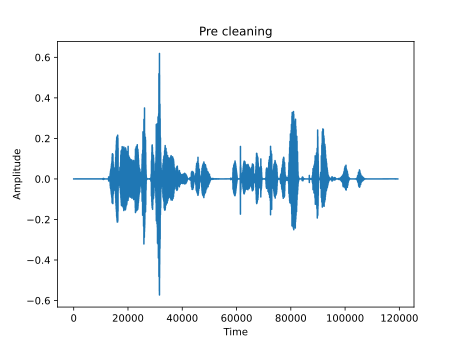
\includegraphics[width=\textwidth]{images/pre_cleaning.png}
    \caption{Pre cleaning shape}
  \end{minipage}
  \hfill
  \begin{minipage}[b]{0.4\textwidth}
    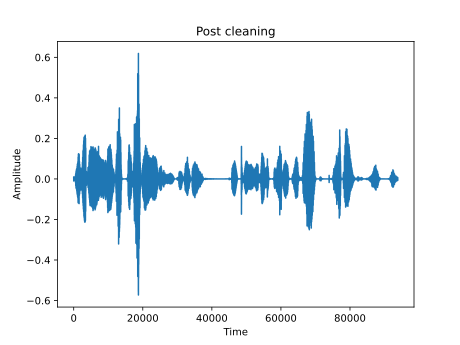
\includegraphics[width=\textwidth]{images/post_cleaning.png}
    \caption{Post cleaning shape}
  \end{minipage}
\end{figure}

\subsection{Statistics}
Before preprocessing our audio data into features for model training, we need to verify that the data is well-balanced across various attributes, such as label distribution, category balance, and uniformity in audio lengths. We looked at three statistics on the data: the number of audio files by language (Figure 3 (a)), the average length of audios by language (Figure 3 (b)), and the total length of audios by language (Figure 3 (c)). 
\begin{figure}[h]
    \centering
    \begin{subfigure}[b]{0.3\textwidth}
        \centering
        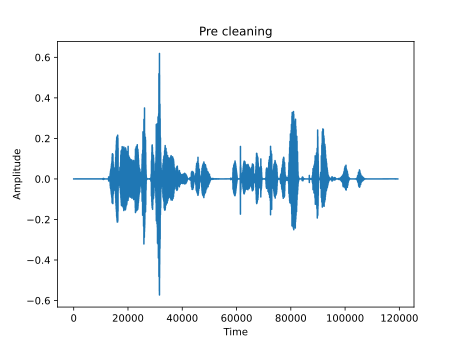
\includegraphics[width=\linewidth]{images/pre_cleaning.png}
        \caption{Figure 1}
        \label{fig:image1}
    \end{subfigure}
    \hfill
    \begin{subfigure}[b]{0.3\textwidth}
        \centering
        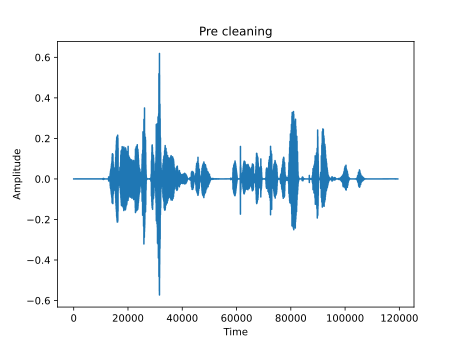
\includegraphics[width=\linewidth]{images/pre_cleaning.png}
        \caption{Figure 2}
        \label{fig:image2}
    \end{subfigure}
    \hfill
    \begin{subfigure}[b]{0.3\textwidth}
        \centering
        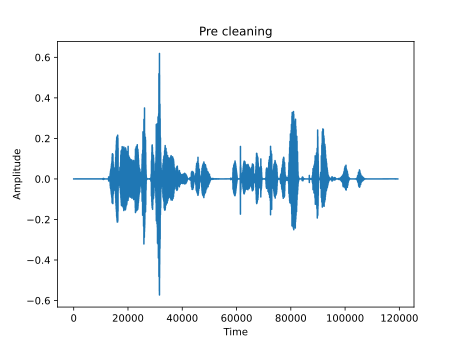
\includegraphics[width=\linewidth]{images/pre_cleaning.png}
        \caption{Figure 3}
        \label{fig:image3}
    \end{subfigure}
    \caption{Three aligned images with individual captions}
    \label{fig:three_images}
\end{figure}\\
By looking at the count, some languages are overrepresented in our data, which is not ideal because it can lead to a model that is biased towards these languages, potentially reducing its performance on underrepresented languages. Furthermore, we can see that the average length of the samples for each are very heterogeneous, ranging from 2 seconds to 5 seconds. This would need to be kept in mind when producing the features from the soundwaves, so the windows properly capture lengths of each file. That being said, by looking at the total length of audios, which is the sum of seconds spoken for each language, we see that the difference between languages is slightly smaller. Overall, we see some unbalancing in our labels. Knowing this, we will need to stratify the dataset when doing the train/test splits so that each language is proportionately represented in the train and test sets, ensuring a more balanced and accurate evaluation of the model's capabilities across all languages.

\subsection{Data Preprocessing}
For the preprocessing of audio data, we use different features which are presented below.

\textbf{MFCCs}:
The Mel Frequency Cepstral Coefficients are criticals in the sense that it allows capturing the different aspects that are unique to each spoken language. It is much easier to differentiate languages by using MFCCs. 
%To obtain the MFCCs, we first found the spectrum of power as a function of our audio file's frequencies from a Fast Fourier Transformation (FFT). Then, it was necessary to find the Mel Filter Banks (MFB) of the spectrum from which we obtain the frequency energies (weighted energy) passing through each filter of the bank. A logarithmic function will be applied to these energies. Finally, by applying a Discrete Cosine Transformation on the log-transformed energies, we obtain the MFCCs.\\

\textbf{Spectral Centroid}: The spectral centroid indicates the center of mass of the sound's spectrum, providing a way to characterize the brightness of a sound. It is calculated as the weighted mean of the frequencies present in the signal, with their magnitudes as the weights.

\textbf{Spectral Rolloff}: The spectral rolloff point indicates the frequency below which a specified percentage of the total energy of the spectrum is located, typically used to distinguish between harmonic (tonal) and noisy sounds. It serves as a way to capture the shape of the sound's spectrum, particularly its high-frequency content.

\textbf{Spectral Bandwidth}: Spectral bandwidth quantifies the width of the frequency band where most of the sound's energy is concentrated, reflecting the sound's perceived texture. It measures the spread of the spectrum around the spectral centroid, indicating the range of significant frequencies that contribute to the sound.

\textbf{Pitch and Intonation Patterns}: Pitch refers to the perceived frequency of a sound, determining the musical note or tone that it corresponds to. Intonation pattern describes the variation of pitch over time within spoken language, contributing to the expression of emotions, questioning, or emphasis in speech.

\textbf{Formant Frequencies}: 
%In audio processing, a formant is a concentration of acoustic energy around a particular frequency in the voice spectrum, associated with the resonant frequencies of the vocal tract. 
Formants play a crucial role in characterizing vowels and certain consonants, greatly influencing speech recognition and synthesis.

\textbf{RMS}: Root Mean Square (RMS) represents the square root of the average power of a signal, providing a measure of its amplitude. It's commonly used to quantify the volume level or energy of an audio signal over time.

\textbf{ZCR}: Zero crossing rate (ZCR) is the rate at which an audio signal changes from positive to negative or back, effectively measuring the number of times the amplitude crosses the zero point. This feature is useful for analyzing the noisiness of a signal and distinguishing between voiced and unvoiced speech.

\section{Methodology}
\subsection{Why supervised Learning ?}
Supervised learning algorithms (SVM and Random forest) are used in this project because unlike unsupervised learning algorithms, supervised algorithms learn the specific characteristics of each language’s phonetic, intonational, and rhythmic properties, leading to highly accurate classification once the model is well-tuned. Unsupervised methods like clustering algorithms (DBscan, K-means or hierarchical clustering) identify groups based on feature similarity but do not inherently know what these groups represent (which language each group corresponds to) which can lead to an ambiguity in cluster interpretation.

Unsupervised algorithms suffer more from the curse of dimensionality than supervised models. In fact, SVMs are more effective even in hight dimension due to the fact that they primarily care about the points closest to the decision boundary (support vectors) rather than the dimensionality of the space. Furthermore, the maximization of the distance between the support vectors and the boundary ensures that the model focuses on the most informative features for classification. This property allows SVM to be less prone to overfitting, a common issue in high-dimensional spaces. Due to the kernel trick, SVMs can also handle non linear decisions which allows them to operate in higher dimensions without directly computing the coordinates in that space unlike unsupervised algorithms (more description about SVM on the section \textbf{4.3}).

In other hands, random forest is based on a set of decision trees which are robust against overfitting because each tree in the forest is bult from a random sample of features, reducing the variance of the set whthout substantially increase the biais. 


\subsection{Dimensionality reduction}
Before applying PCA or MDS, we wanted to see the relationship between features i.e. how strongly they are correlated. This correlation study would guide us in the dimensionality reduction algorithm we choose to apply to our data. If some features are strongly correlated, PCA would be pertinent to be applied, as some features are linearly related. Even though our correlation study gave us pretty strong evidence of non-linear relationship between our features (meaning that MDS might be a better suit for our dataset), we opted to reduce dimensionality using PCA due to insufficient computing and memory. After applying PCA, with a maintained variance of $99\%$, we have $112$ features from the $151$ intial features. This means that the first $112$ principal components of the covariance matrix $\Sigma \in \mathbb{R}^{151 \times 151}$ , where $\forall i \in 1, \ldots, 151 \quad \forall j \in 1, \ldots, 151 \quad \sigma_{ij} \in \Sigma, \sigma_{ij} = COV(x_i, x_j)$, capture $99\%$ of the original dataset.

\subsection{Support Vector Machine}
For this project, we use the library \textit{SVC} from \textit{sklearn}. This library use a non-linear SVM with a soft margin. Non-linear SVM with a soft margin is particularly useful when dealing with data that cannot be linearly separated in the original feature space (which is the case in our situation). The inclusion of slack variables, \(\xi_i\), allows some data points to be on the incorrect side of the margin, providing a balance between the complexity of the model and its error minimization.\\

\textbf{Mathematics formulation:}

For a dataset $X \in \R^{n \times p}$ and a vector $y \in \{-1, 1\}^n$, the objective is to find $w$ such that the values returned by the functions $f(X) = sign(w^T\phi(x) + b)$ are correct for most samples.\\
SVC resolve the following primal problem : \(
\min_{w, b, \boldsymbol{\xi}} \left( \frac{1}{2} w^T w + \beta \sum_{i=1}^{n} \xi_i \right)
\) 
subject to:\\
\( y_i (w^T \phi(x_i) + b) \geq 1 - \xi_i\), \(\xi_i \geq 0, \quad \forall i\).
By using lagrange multiplier, we obtains the dual :\(\min_{\alpha} \frac{1}{2} \alpha^T Q \alpha - \mathbf{1}^T \alpha
\) subject to: \(y^T \alpha = 0\), \(0 \leq \alpha_i \leq \beta, i=1,...,n\) with $Q$ an $n$ by $n$ positive semidefinite matrix, $Q_{ij} \equiv y_iy_jK(x_i, x_j)$, where $K(x_i, x_j) = \phi(x_i)^T\phi(x_j)$ is the kernel. 

After the optimisation is done, the output for the decision function for $X$ is :\(\sum_{i\in SV} y_i\alpha_i K(x_i, x) + b\)
where $SV$, represent the support vectors (the points that lies within the margin).

\textbf{Hyperparameters:}


\begin{comment}
\textbf{Kernel Function}\\
Common choices for the kernel function \(K\) include:
- Polynomial: \(K(\mathbf{x}_i, \mathbf{x}_j) = (\gamma \mathbf{x}_i^T \mathbf{x}_j + r)^d\),
- Radial Basis Function (RBF): \(K(\mathbf{x}_i, \mathbf{x}_j) = \exp(-\gamma \|\mathbf{x}_i - \mathbf{x}_j\|^2)\),
- Sigmoid: \(K(\mathbf{x}_i, \mathbf{x}_j) = \tanh(\gamma \mathbf{x}_i^T \mathbf{x}_j + r)\).
\(\gamma\), \(r\), and \(d\) are parameters that can be tuned according to the specific data and problem requirements.  
\end{comment}


\subsection{Random Forest}

\section{Results}
\subsection{PCA}
 
\subsection{SVM vs Random Forest Classifier}

\section{Conclusion}

\section{References}
\begin{itemize}
    \item \href{https://huggingface.co/datasets/common_language}{Data Source}
    \item \href{https://ietresearch.onlinelibrary.wiley.com/doi/full/10.1049/tje2.12082#:~:text=All\%20performance\%20metrics\%20gave\%20the,studies\%20use\%20only\%2013\%20MFCCs}{Number of MFCCs used in the code}
    \item \href{https://scikit-learn.org/stable/modules/svm.html#svm-kernels}{Source for non linear SVM with soft margin}
\end{itemize}

\end{document}
